\documentclass[a4paper]{scrartcl}
\usepackage{lmodern} % latin modern font family
\usepackage[ngerman]{babel}
\usepackage{biblatex}
\bibliography{sources.bib}
% \usepackage{babelbib} % for german bibliography style babplain-fl
\usepackage{csquotes} % language specific quotes
\setlength{\parindent}{0pt} % no indentation new paragraph

\usepackage{amsmath} % math-stuff
\usepackage{amssymb} % math-symbols
\usepackage{amsthm} % qed symbol

% \usepackage{mathtools} % better alignment in matrix with optional args
\usepackage{enumitem} % a,b,c enumerate
% \usepackage{nicefrac} % inline fractions
\usepackage{url} % nice urls
\usepackage{hyperref} % clickable urls

\usepackage{listings} % source code
\usepackage{fontspec} % for custom font selection
\newfontfamily\lstfamily{DejaVuSansMono} % defines a new font family used in listings

\usepackage{xcolor} % for custom colors
\definecolor{darkgreen}{rgb}{0, 0.65, 0}
\definecolor{codepurple}{rgb}{0.58, 0, 0.82}
\definecolor{codebackground}{rgb}{0.98, 0.98, 0.98}
\lstdefinestyle{mystyle}{
    backgroundcolor = \color{codebackground},
    commentstyle = \color{darkgreen},
    keywordstyle = \color{blue},
    stringstyle = \color{orange},
    basicstyle = \scriptsize\lstfamily,
    showstringspaces = false
}
\lstset{style = mystyle}

\usepackage{graphicx} % inclusion of external graphics with \includegraphics
\usepackage{float} % figure placements

\usepackage[ngerman, noabbrev]{cleveref} % referenced type name included in ref

\title{PetriCheck}
\author{j-hap}

\begin{document}
\maketitle
\pagebreak
\tableofcontents
\pagebreak
\section{Einleitung}
Das hier vorgestellte Programm zur interaktiven und grafischen Analyse von
Petri-Netzen, genannt \emph{PetriCheck}, wurde im Rahmen des Kurses 1584 der
Fernuniversität Hagen erarbeitet. PetriCheck ermöglicht den Import von
Petri-Netzen auf Basis von Dateien in der Petri Net Modeling Language (PNML). Neben
dem interaktiven Schalten von Transitionen bietet es die automatisierte Analyse
von beliebig vielen PNML-Dateien bzw. den darin enthaltenen Petri-Netzen.

Das vorliegende Dokument geht auf die Implementierung der geforderten
Analysemethoden sowie die über die Aufgabenstellungen hinausgehenden
Funktionalitäten ein.

Die geschlechtsneutrale Sprache in diesem Dokument geht auf eine Idee des
Aktionskünstler Hermes Phettberg zurück \cite{arzty}.
\section{Bedienungsanleitung}
Neben den in der Aufgabenstellung geforderten Funktionen der Anwendung wurden
einige vorgeschlagene Zusatzfunktionen implementiert:
\begin{itemize}
  \item Erkennung von Unbeschränktheit beim Aufbau des pEG
  \item Multiple Document Interface
  \item Übersichtliche Darstellung des pEG
\end{itemize}
Diese und darüber hinausgehende Funktionen der Anwendung werden in den folgenden
Unterabschnitten beschrieben.

\subsection{Tab Interface}
Die Untersuchung und Bearbeitung von mehreren Petri-Netzen gleichzeitig ist mit
Petri-Check durch ein Tab Interface ermöglicht. Jedes Petri-Netz wird dabei in
einem eigenen Tab, wie in modernen Web-Browsern, angezeigt.

Nach dem Start von PetriCheck wird dem Anwendy die in \cref{img:default_window}
gezeigte Bedienoberfläche präsentiert.

\begin{figure}[H]
  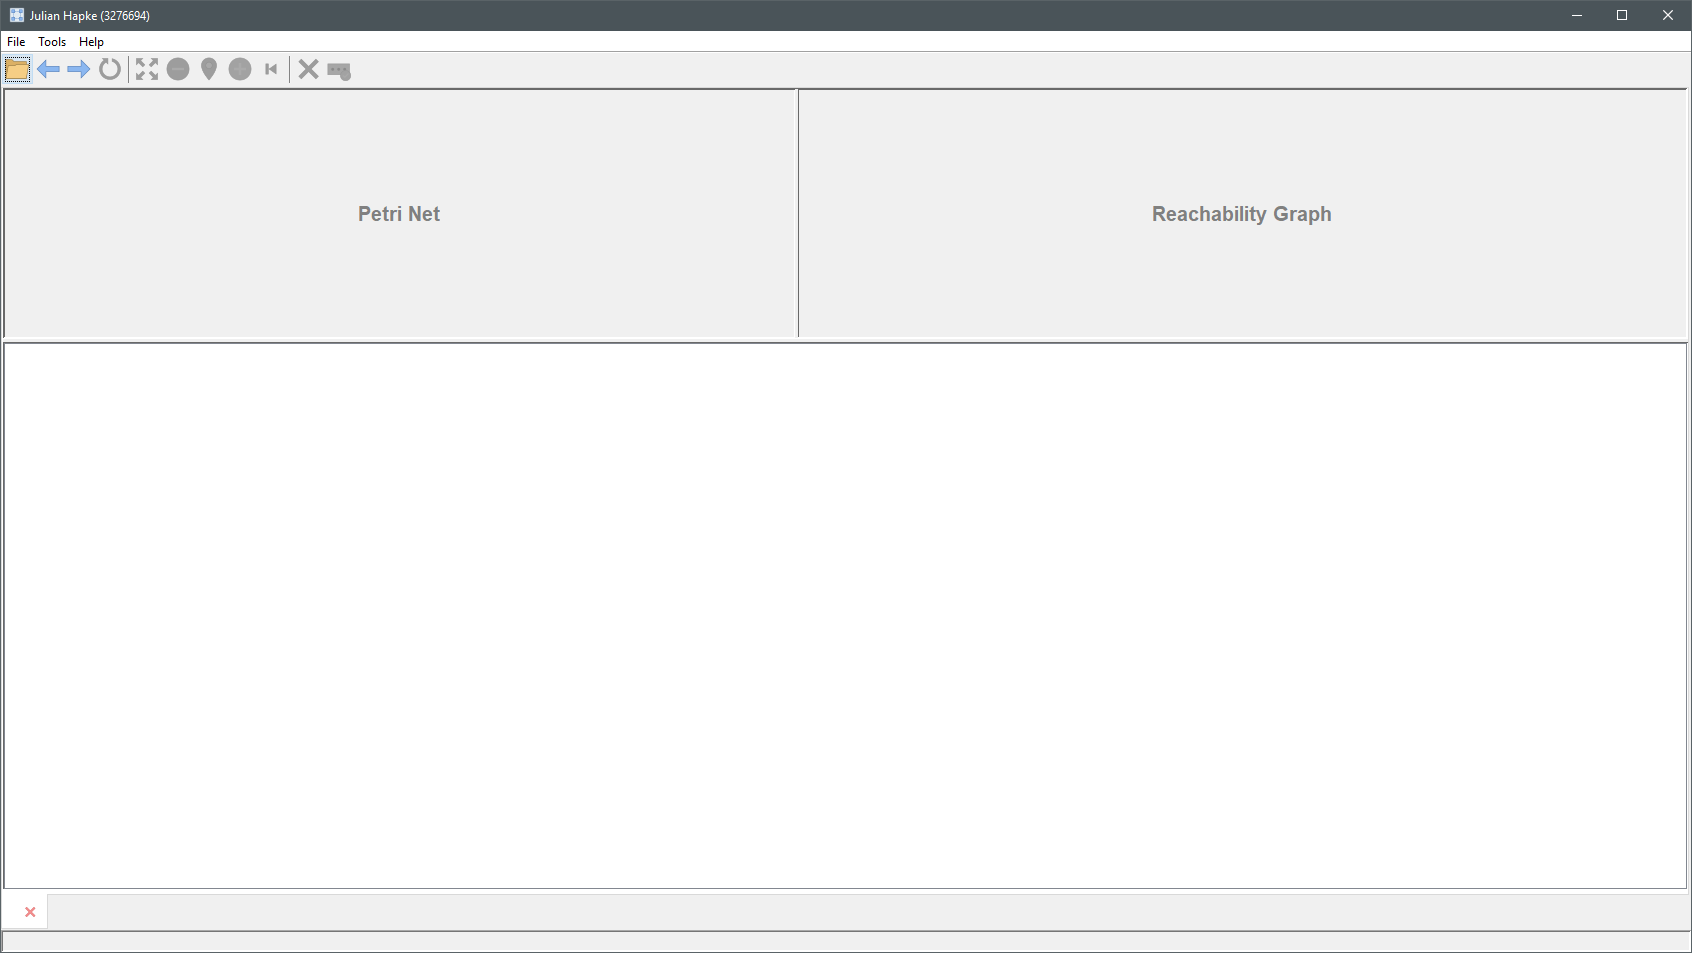
\includegraphics[width=\textwidth]{../img/default_window.png}
  \caption{Programmfenster nach dem Start}
  \label{img:default_window}
\end{figure}

Es ist kein Petri-Netz geöffnet, es wird aber ein Default-Tab angeboten, der
über einen vergrößerten Textausgabebereich verfügt. Dieser Bereich ist für die
Ausgabe der Ergebnisse einer Beschränktheitsanalyse mehrerer Dateien vorgesehen,
die auch ausgeführt werden kann, wenn kein Petri-Netz geöffnet ist.

Wird über die Standardfunktionen nun ein Petri-Netz geöffnet, so wird der
Default-Tab ersetzt, sofern in ihm keine Informationen im Textausgabebereich
vorhanden sind. Andersfalls wird ein zusätzlicher Tab erstellt.

Wegen der Möglichkeit mehrere Dateien gleichzeitig zu öffnen, ist in jedem
Dateiauswahldialog eine Mehrfachauswahl von PNML-Dateien möglich. Jede Datei
wird dann in einem eigenen Tab geöffnet. Ist eine ausgewählte Datei bereits
geöffnet, wird sie nicht erneut geöffnet, sondern der mit dieser Datei
assoziierte Tab aktiviert. Das Inhalts-Panel des Tabs wird durch die Klasse
\texttt{SwingTab} implementiert.

Um einen Tab und das darin enthaltene Petri-Netz zu schließen, existiert
einerseits der Menüpunkt \emph{Datei $\rightarrow$ Schließen}. Andererseits
verfügt jeder Tab am unteren Rand rechts neben seinem Titel über einen kleinen
\raisebox{-2pt}{
\includegraphics{../../src/main/resources/icons/icons8-delete-12.png}}
Button. Ein Klick auf diesen Button verursacht ebenfalls das Schließen des
entsprechenden Tabs. Wird jedoch der letzte Tab geschlossen, wird standardmäßig
ein leerer Default-Tab, wie in \cref{img:default_window} dargestellt, erzeugt,
um eine Ausgabemöglichkeit für die Stapelverarbeitung mehrerer Dateien zu haben.

Die Verwaltung der Tabs und die Assiziation der Tabs mit den geöffneren Dateien
übernimmt ein Objekt der Klasse \texttt{TabManager} bzw. ein Objekt der auf das
Swing-Framework spezialisierten Klasse \texttt{SwingTabManager}. Da keine Datei
doppelt geöffnet werden kann, verwaltet ein \texttt{SwingTabManager} die
offnenen Tabs in Maps, um Tabs mit absoluten Dateinamen und umgekehrt zu
assizieren. Außerdem benachritigt ein \texttt{TabManager} eventuell vorhandene
Listener-Objekte über ein umschalten des aktiven Tabs durch den Nutzer.

Zusätzlich kümmert sich der TabManager darum, dass im globalen Logger das
Textfeld des jeweils aktiven Tab als Ausgabe genutzt wird.

\subsection{Mehrsprachigkeit}
Die Sprache der Bedienoberfläche kann verändert werden (siehe
\cref{sec:settings}). Beim ersten Start der Anwendung, wenn noch keine
Einstellung vorhanden ist, wird versucht die Sprache des Betriebssystems
einzustellen. Sind für diese Sprache keine Übersetzungsdateien vorhanden, wird
eine Oberfläche mit englischen Texten erstellt.

\subsection{Look and Feel}
Um eine im Vergleich zum Betriebssystem einheitliche Optik zu erreichen,
versucht PetriCheck das Look-and-Feel des Swing Frameworks an das des
Betriebssystems anzupassen. Nur wenn diese Anpassung scheitert, weil Swing z.B.
das aktuelle Betriebssystem nicht unterstützt, dient die etwas historisch
anmutende Standardoptik von Swing als Rückfallebene.

\subsection{Kontinuierliche Beschränktheitsanalyse}
Ein Anwendy kann während des interaktiven Schaltens über die Unbeschränktheit
des aktuellen Petri-Netzes informiert werden. Um diese Warnung nicht zu
erhalten, kann diese in den Einstellungen (siehe \cref{sec:settings})
deaktiviert werden. Die Warnung erscheint nur einmalig und nicht bei jedem
Schalten nachdem die Unbeschränktheit erkannt wurde. Wird die initiale
Markierung der Petri-Netzes verändert oder das Petri-Netz erneut aus der Datei
eingelesen, wird die Warnung ggf. erneut ausgegeben.

Implementiert ist diese Funktionalität im \texttt{PetriNetController}, damit die
Warnung nur während des interaktiven Schaltens des Netzes emittiert wird.

\subsection{Hierarchisches Layout des Erreichbarkeitsgraphen}
Neben dem automatischen \emph{SpringBox} Layout der GraphStream Bibliothek, kann
auf die simple Implementierung eines hierarchischen Layouts umgeschaltet werden
(siehe \cref{sec:settings}). Dieses hierarchische Layout stellt einen Graphen
mit einem festen Ursprungknoten (oben) in verschiedenen Ebenen dar. Die Ebene
eines Knotens wird hierbei über die kürzeste Verbindung vom Ursprungsknoten zu
diesem Knoten festgelegt. Wird im Verlauf des Aufbaus des partiellen
Erreichbarkeitsgraphen eine weitere Kante hinzugefügt, sodass ein kürzerer Pfad
vom Ursprungknoten zu einem Knoten entsteht, so wird dieser Zielknoten in der
Hierarchie weiter nach oben gelegt. Innerhalb einer Hierarchieebene werden die
Knoten in der Reihenfolge des Hinzufügens zu dieser Ebene äquidistant
angeordnet. In \cref{img:ex178_hierarchy} ist beispielhaft die Darstellung des
Erreichbarkeitsgraphen mit dem \emph{HierarchyLayout} dargestellt.

\begin{figure}[ht!]
  \centering
  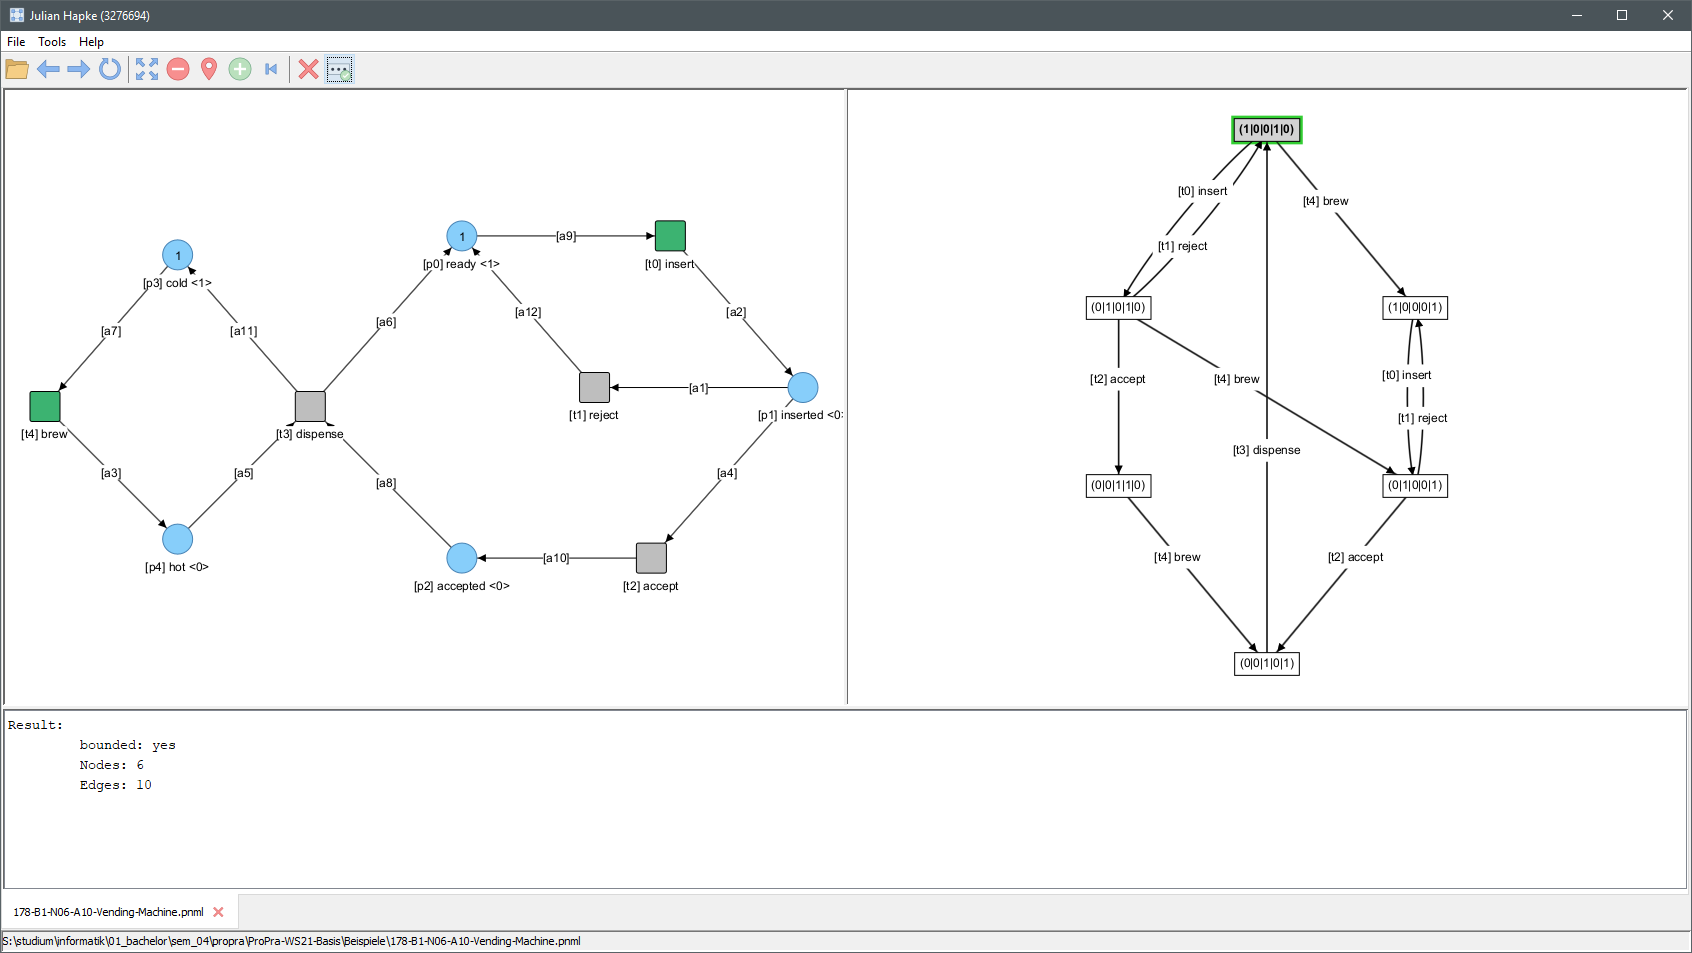
\includegraphics[width=\textwidth]{../img/Screenshot_178_hierarchy_layout.png}
  \caption{Beispieldatei 178 nach Beschränktheitsanalyse mit hierarchischem Layout}
  \label{img:ex178_hierarchy}
\end{figure}

\subsection{Einstellungen}
\label{sec:settings}
Nach dem Aufruf des Menüpunkt \emph{Extras $\rightarrow$ Einstellungen\ldots}
wird der in \cref{img:settings} dargestellt Dialog gezeigt.

\begin{figure}[H]
  \centering
  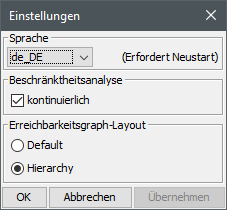
\includegraphics[width=0.3\textwidth]{../img/settings.png}
  \caption{Programmfenster nach dem Start}
  \label{img:settings}
\end{figure}

In diesem Dialog kann die Sprache der Oberfläche, die Warnung vor
Unbeschränktheit bei interaktivem Aufbau des Erreichbarkeitsgraphen und das
Layout der Darstellung des Erreichbarkeitsgraphen eingestellt werden. Die
Änderung der Sprache der Oberfläche bedarf eines Neustarts der Anwendung. Die
Änderung des Layouts des Erreichbarkeitsgraphen bedarf einer Neuerstellung des
Graphen, entweder durch Ausführen der Beschränktheitsanalyse oder Löschen des
aktuellen partiellen Erreichbarkeitsgraphen.

\subsection{Erweiterte Mausbedienung}
Wie in der Aufgabenstellung gefordert, kann mit dem Mausrad in die Ansicht eines
Graphen gezoomt werden. Neben der Änderung des Zoom-Levels, wird die Mitte der
Ansicht derart verschoben, dass der Mauszeiger seine Position relativ zum
Graphen beibehält. Dieses Verhalten sind Anwendys zum Beispiel in Programmen der
Bildbetrachtung und -bearbeitung gewohnt.

Desweiteren wurde dafür gesorgt, dass Verschieben eines Graphen ebenfalls mit
der Maus möglich ist. Wird die rechter Maustaste auf einem Graphen geklickt und
die Maus bewegt, so wird der darunterliegende Graph mit verschoben.
\section{Programmstruktur}
\label{sec:struct}

In diesem Abschnitt wird auf die Implementierung der Modell-Klassen und die
darin verwendeten Datenstrukturen eingegangen.

\subsection{PetriNet}

Die Klasse \texttt{PetriNet} bildet die Modell-Repräsentation eines Petri-Netzes
in PetriCheck dar. Wegen der Einzigartigkeit der Element-IDs werden die Stellen,
Transitionen und Kanten als eigene Objekte jeweils in Java \texttt{Map}s
organisiert. Dies ermöglicht schnellen und komfortablen Zugriff auf die Elemente
des Netzes mittels ihrer ID.

Um sicherzustellen, dass jede ID einzigartig ist ist, wird bei jedem Hinzufügen
eines neuen Elementes geprüft, ob die ID des zu erzeugenden Elementes
einzigartig ist. Hierfür wird ein \texttt{Set} von IDs befüllt und vor jedem
Einfügen geprüft, ob die neue Element-ID in diesem Netz schon in Verwendung ist.

Wird die Einzigartigkeitsbedingung verletzt, so informiert das PetriNet die
aufrufende Methode mittels Exception darüber. In PetriCheck erfolgt der Aufbau
des Petri-Netzes ausschließlich auf Dateibasis. Der dafür verwendete
\texttt{SimplePnmlParser} kann durch Abfangen dieser Exceptions den Anwender
über Fehldefinitionen innerhalb der PNML-Datei über Logger-Ausgaben informieren.

Die Kanten werden zwar auch innerhalb des \texttt{PetriNet} Objektes gehalten,
allerdings dienen diese nur dazu eine grafische Repräsentation der Kanten zu
erstellen. Die eigentliche Schaltlogik ist auf Elementebene implementiert.
Stellen und Transitionen sind als eigene Klassen implementiert. Jeder Transition
werden beim Hinzufügen der Kanten zum Petri-Netz ihre Vorgänger- und
Nachfolger-Stellen bekannt gemacht. Das Petri-Netz selbst gibt zum Schalten
einer Transition nur der zu schaltenen Transition Bescheid. Die Umverteilung von
Tokens geschieht dann auf Element-Ebene.

\subsection{ReachabilityGraph}

Die Klasse \texttt{ReachabilityGraph} bildet die Modell-Repräsentation eines
Erreichbarkeitsgraphen in PetriCheck dar.

Wegen der einfacheren Synchronisation erstellt jedes \texttt{PetriNet} Objekt
bei seiner Erstellung direkt ein \texttt{ReachabilityGraph}-Objekt. So kann
sichergestellt werden, dass jedes Petri-Netz stets einen eigenen
Erreichbarkeitsgraphen pflegt und die Schalthistorie verfolgt wird.

Die Knoten des Erreichbarkeitsgraphen werden durch
\texttt{LinkedMarking}-Objekte gebildet. Dies ist eine Subklasse der
\texttt{Marking}-Klasse. Ein \texttt{Marking}-Objekt stellt eine Markierung
eines Petri-Netzes dar. Hierbei wird die Anzahl der Tokens einer jeden Stelle
durch eine einfache Ganzzahl in einem Array repräsentiert. Die Ordnung in diesem
Array entspricht der alphabetischen Ordnung der IDs der Stellen. Zwei
\texttt{Marking}s mit derselben Markierung gibt den gleichen Hash-Wert aus.
Ebenso bezieht sich der Vergleich mit der \texttt{equals}-Methode ausschließlich
auf die repräsentierte Markierung. Dies vereinfacht die Handhabung von zwei
unterschiedlichen \texttt{Marking}s, die aber die selbe Markierung des
Petri-Netzes repräsentieren.

Ein \texttt{LinkedMarking} enthält neben den geerbten Attributen des
\texttt{Marking}s die Verbindungen zu anderen \texttt{LinkedMarking}s, sowohl
Vorgänger als auch Nachfolger. Da die Kanten in einem Erreichbarkeitsgraphen
gelabelt sind, dient die generische Klasse \texttt{Edge} als Repräsentation
einer gelabelten Kante. Jedes \texttt{Edge}-Objekt enthält den Namen der Kante
sowie den Ursprungs-/Zielknoten der Kante, je nachdem wie sie verwendet wird.
Die Nachbarn eines \texttt{LinkedMarking}s werden also zwei \texttt{Set}s von
\texttt{Edge}-Objekten gehalten. Dies ermöglicht die Identifikation von
Vorgänger- und Nachfolgermarkierungen, was beim Aufbau des
Erreichbarkeitsgraphen als auch bei der Beschränktheitsanalyse dienlich ist
(siehe \cref{sec:algo}).

Wie bei den \texttt{Marking}-Objekten gelten zwei Edges als gleich, wenn sie das
gleiche Label und den gleichen Endknoten haben. Zwei Edge-Objekte liefern dann
also auch den gleichen Hash-Wert, der zur Indentifikation in \texttt{HashSet}s
genutzt wird. Dies ermöglicht die einfache Kontrolle, ob im Petri-Netz
geschaltete Trasitionen schon im Netz vorhanden sind, auch wenn diese Kante
durch ein separates Objekt repräsentiert wird.

\subsection{UI-Actions}
Die Implementierung der dem Anwender angebotenen Aktionen in der grafischen
Bedienoberfläche (GUI) ist mit möglichst geringer Code-Duplikation umgesetzt. Es
können einige Aktionen in der Oberfläche an mehreren Stellen ausgelöst werden,
zum Beispiel im Menüband als auch in der Toolbar. Es soll aber nur eine
Repräsentation dieser Aktion existieren. Hierfür werden die \texttt{Action}s als
Eigenschaften von \texttt{Enum}-Objekten in der \texttt{MainViewAction}
Enumeration gehalten. Jedes Objekt dieser Aufzählung wird bei der Erstellung mit
einem anzuzeigenden Befehlstext, einem Hinweistext (Tooltip) und einem Element
der \texttt{UiIcon}-Enumeration versehen. Innerhalb eines
\texttt{UiIcon}-Objekts sind Icons in zwei Größen eingebettet, ein Icon für die
Darstellung eines Toolbar-Buttons und ein Icon für die Visualisierung innerhalb
des Anwendungsmenüs. Diese Icons werden an die entsprechenden Stellen in der
Action gesetzt, sodass das Swing Framework das jeweils geeignete Icon in der
Oberfläche darstellt.

Die unterhalb der einzelnen \texttt{MainViewAction}-Einträgen liegenden
\texttt{Action}s werden beim Aufbau der Bedienoberfläche an den jeweilgen
Stellen eingesetzt. Wird nun eine dieser Action aus dem GUI heraus getriggert,
so erfolgt eine Weiterleitung der Aktion an ein zentrales Mediator-Objekt, das
im Vorfeld der \texttt{MainViewAction}-Aufzählung mitgeteilt wurde.

Bei der Weiterleitung wird allerdings der ursprüngliche Auslöser der Aktion, die
\texttt{Action} eines \texttt{MainViewAction}-Objekts, durch das
\texttt{MainViewAction}-Objekt selbst ersetzt. Dies ermöglicht eine komfortable
Entscheidung mittels \texttt{switch}-Statements darüber, welche Aktion im
Mediator-Objekt ausgelöst werden soll.

Die Umsetztung sowohl der \texttt{MainViewAction}- als auch der
\texttt{UiIcon}-Objekte in Aufzählungen erlaubt die einfache Verwaltung aller
verfügbaren Aktionen an zentraler Stelle bei geringem Code-Umfang.

Die Rolle des Mediator-Objekts nimmt die \texttt{MainController}-Klasse ein.
\section{Beschränktheits-Algorithmus}
\label{sec:algo}

\subsection{Beschränktheit des Erreichbarkeitsgraphen}
Wie in \cref{sec:struct} beschrieben, hält jedes Petri-Netz seinen eigenen
Erreichbarkeitsgraphen als Attribut. Beim Hinzufügen einer neuen Markierung in
den Erreichbarkeitsgraphen, wird geprüft, ob es eine Markierung auf dem Weg zur
Wurzel-Markierung gibt, die die m $\leftrightarrow$ m' Relation verletzt. Diese
Pfade werden mittels Breitensuche abgeschritten. Hierbei ist eine rückwärts
gerichtete Breitensuche mittelt der in einem \texttt{LinkedMarking} gehaltenen
\texttt{Edge}s zu den Vorgänger-Markierungen einfach implementierbar.

Sei \texttt{get\_predecessors} eine Methode um die Vorgänger-Knoten eines Knoten
in einem Erreichbarkeitsgraphen zu erhalten. Der \texttt{\textgreater}-Operator
führe für zwei Markierungen A und B den elementweisen Vergleich der Token-Anzahl
an jedem Index aus und gibt \texttt{true} zurück, wenn A an mindestens einer
Position eine größere Token-Anzahl als B enthält und an allen anderen Stellen
die Anzahl der Tokens gleich groß ist. %
Die Prüfung der m $\leftrightarrow$ m' Relation stellt
sich dann in Pseudocode wie folgt dar, wobei davon ausgegangen wird, dass die
Startmarkierung der Suche im Erreichbarkeitsgraphen vorhanden ist.

\begin{lstlisting}[language=python, morekeywords={do, algorithm, then}]
  algorithm check_bounded(r_graph, start_marking)
    visited_markings = Set() # of Markings
    visited_markings.add(start_marking)
    queue = DoubleEndedQueue()
    start_node = r_graph.get_node(start_marking)
    queue.append(start_node.get_predecessors())
    while not queue.is_empty() do
      other_node = queue.pop_first()
      if (visited_markings.contains(other)) then
        continue
      if (start_marking > other) then
        return false
      q.append(other.get_predecessors())
      visited_markings.add(other)
    return true
\end{lstlisting}

\subsection{Beschränktheit des Petri-Netzes}
Um die (Un)Beschränktheit eines Petri-Netzes festzustellen, werden bei der
Beschränktheitsanalyse so lang Transitionen geschaltet, bis entweder
\begin{itemize}
  \item alle möglichen Pfade durch das Petri-Netz beschritten wurden und keine
        aktiven Transitionen mehr vorhanden sind oder
  \item beim Aufbau des Erreichbarkeitsgraphen die Unbeschränktheit des Netzes
        festgestellt wurde.
\end{itemize}

Um alle möglichen Pfade in einem Petri-Netz zu beschreiten, wird in PetriCheck
eine Tiefensuche im Petri-Netz verwendet. Hierfür verfügt die Implementierung
des Petri-Netzes über eine Hilfsmethode, die eine Liste der gerade aktiven
Transitionen ausgeben kann:

\begin{lstlisting}[language=python, morekeywords={do, algorithm, then}]
  algorithm get_active_transitions(petri_net)
    output = []
    for transition in petri_net.transitions do
      if transition.is_active() then
        output.append(transition)
    return output
\end{lstlisting}

Im initialen Schritt des Algorithmus wird das Petri-Netz auf seine
Ausgangsmarkierung zurückgesetzt und der Erreichbarkeitsgraph reinitialisiert.
Hierbei werden alle bisherigen eventuell durch interaktives Schalten von
Transitionen vorhandenen Markierungen und Kanten gelöscht und nur der
Wurzelknoten, die Ausgangsmarkierung, hinzugefügt. Anschließend kann die rekursiv
formulierte Tiefensuche gestartet werden.

\begin{lstlisting}[language=python, morekeywords={do, algorithm, then}]
  algorithm is_bounded(petri_net)
    petri_net.reset()
    petri_net.r_graph.initialize()
    return is_bounded_rec(petri_net)
\end{lstlisting}

In der Tiefensuche wird zuerst die aktuelle Markierung gesichert, damit sie nach
dem Schalten einer Transition wiederhergestellt werden kann. Der rekursive
Abstieg erfolgt in der if-Bedingung, um beim Auffinden der ersten Verletzung der
m $\leftrightarrow$ m' Relation die Rekursion zu beenden. Der rekursive
Algorithmus lautet in Pseudocode:

\begin{lstlisting}[language=python, morekeywords={do, algorithm, then}]
  algorithm is_bounded_rec(petri_net)
    last_marking = petri_net.get_marking()
    for transition in get_active_transitions(petri_net) do
      # this call adds marking to r_graph and checks boundedness
      petri_net.trigger_transition(transition)
      if not petri_net.r_graph.is_bounded or not is_bounded_rec(petri_net) then
        return false
      petri_net.set_marking(last_marking)
    return true
\end{lstlisting}

Neben diesen Schritten wird in der Implementierung in PetriCheck noch der
aktuell beschrittene Pfad dokumentiert und zwei ggf. gefundene in m
$\leftrightarrow$ m' Relation stehende Markierungen für die Ausgabe gesichert.

Die Ansicht des Programms nach der Beschränktheitsanalyse der Beispieldatei 276 zeigt \cref{img:ex276_default}.

\begin{figure}[H]
  \includegraphics[width=\textwidth]{../img/Screenshot_276_default_layout2.png}
  \caption{Beispieldatei 276 nach der Beschränktheitsanalyse}
  \label{img:ex276_default}
\end{figure}

% \clearpage % forces all unset pictures before bibliography
\printbibliography
\end{document}
